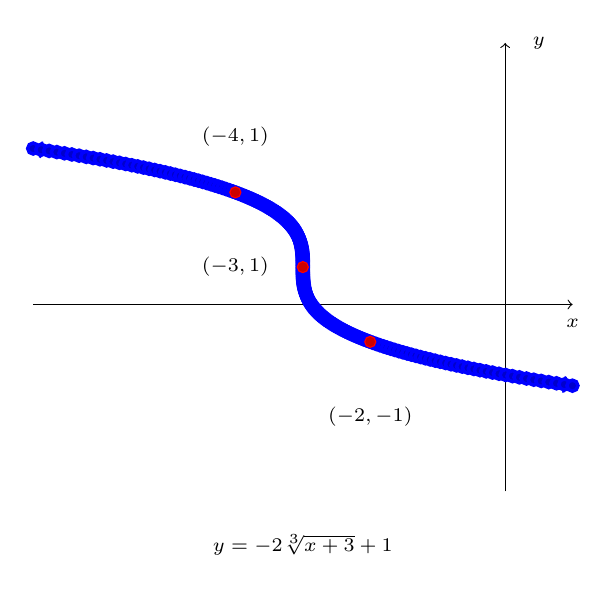
\begin{tikzpicture}
\begin{axis}[
  xmin=-7, xmax=1,
  ymin=-5, ymax=7,
  axis lines=middle,
  axis line style={->},
  ticks=none,
  clip=false
]
\node at (axis cs:1,-0.5){\scriptsize $x$};
\node at (axis cs:0.5,7){\scriptsize $y$};
\node at (axis cs:-2,-3){\scriptsize $(-2,-1)$};
\node at (axis cs:-4,1){\scriptsize $(-3,1)$};
\node at (axis cs:-4,4.5){\scriptsize $(-4,1)$};

\addplot+[domain=-1.587:1.587, samples=200, smooth, line width=1.25pt, <->, variable=\t, parametric]
  ({\t^3-3},{1-2*\t});

\addplot+[only marks, mark=*, mark size=2pt] coordinates {(-2,-1) (-3,1) (-4,3)};

% Caption
\node at (rel axis cs:0.5,-0.12){\scriptsize $y=-2\sqrt[3]{x+3}+1$};
\end{axis}
\end{tikzpicture}